% !TEX TS-program = pdflatex
% !TEX encoding = UTF-8 Unicode

% This is a simple template for a LaTeX document using the "article" class.
% See "book", "report", "letter" for other types of document.

\documentclass[11pt]{article} % use larger type; default would be 10pt

\usepackage[utf8]{inputenc} % set input encoding (not needed with XeLaTeX)

%%% Examples of Article customizations
% These packages are optional, depending whether you want the features they provide.
% See the LaTeX Companion or other references for full information.

%%% PAGE DIMENSIONS
\usepackage{geometry} % to change the page dimensions
\geometry{a4paper} % or letterpaper (US) or a5paper or....
\geometry{margin=0.5in} % for example, change the margins to 2 inches all round
% \geometry{landscape} % set up the page for landscape
%   read geometry.pdf for detailed page layout information

\usepackage{graphicx} % support the \includegraphics command and options

% \usepackage[parfill]{parskip} % Activate to begin paragraphs with an empty line rather than an indent

%%% PACKAGES
\usepackage{booktabs} % for much better looking tables
\usepackage{array} % for better arrays (eg matrices) in maths
\usepackage{paralist} % very flexible & customisable lists (eg. enumerate/itemize, etc.)
\usepackage{verbatim} % adds environment for commenting out blocks of text & for better verbatim
\usepackage{subfig} % make it possible to include more than one captioned figure/table in a single float
% These packages are all incorporated in the memoir class to one degree or another...

%%% HEADERS & FOOTERS
\usepackage{fancyhdr} % This should be set AFTER setting up the page geometry
\pagestyle{fancy} % options: empty , plain , fancy
\renewcommand{\headrulewidth}{0pt} % customise the layout...
\lhead{}\chead{}\rhead{}
\lfoot{}\cfoot{\thepage}\rfoot{}

%%% SECTION TITLE APPEARANCE
\usepackage{sectsty}
\allsectionsfont{\sffamily\mdseries\upshape} % (See the fntguide.pdf for font help)
% (This matches ConTeXt defaults)

%%% ToC (table of contents) APPEARANCE
\usepackage[nottoc,notlof,notlot]{tocbibind} % Put the bibliography in the ToC
\usepackage[titles,subfigure]{tocloft} % Alter the style of the Table of Contents
\renewcommand{\cftsecfont}{\rmfamily\mdseries\upshape}
\renewcommand{\cftsecpagefont}{\rmfamily\mdseries\upshape} % No bold!

%%% END Article customizations

%%% The "real" document content comes below...

\title{Week 8 Assignment}
\author{Efeosa Eguavoen - 17324649}
%\date{} % Activate to display a given date or no date (if empty),
         % otherwise the current date is printed 

\begin{document}
\maketitle

\section{i}
\subsection{A}
To perform the convolve the kernel, I first checked that the dimensions of the kernel are smaller or equal to the dimensions of the input layer.
\begin{verbatim}
def convolver(input_array, kernel):
    k_width = len(kernel)
    k_height = len(kernel[0])
    if k_height <= len(input_array[0]) and k_width <= len(input_array):
\end{verbatim}
I then calculated how many times the kernel will need to 'shift' to convolve correctly.  \begin{verbatim}
shift_len = len(input_array) - k_width + 1
\end{verbatim}
Following I created an output array to hold all the values of the output that I would reform later.  I then created 4 nested for loops, with the outer 2 shifting the kernel across horizontally all the way then drops down one layer vertically and shifts again etc till it's covered the whole input.  
\begin{verbatim}
out_arr = []
        for i in range(shift_len):
            for s in range(shift_len):
                temp = 0
\end{verbatim}
The 2 inner arrays are for indexing across the kernel and multiplying by the corresponding element of the input layer.  I get the correct input array element by offsetting by what row and column it is. \begin{verbatim}
for f in range(k_width):
                    for j in range(k_height):
                        kern = kernel[f][j]
                        inp = input_array[f + i][j + s]
                        temp += kern * inp
                   out_arr.append(temp)
\end{verbatim}
Finally I reshaped the output array into the shape that would be expected given the kernel and input array \begin{verbatim}
	    offset = (len(input_array) - k_width) + 1
        output = [out_arr[i:i + offset] for i in range(0, len(out_arr), offset)]
        return output
\end{verbatim}
\subsection{B}
Original Image: \includegraphics[scale=1]{rsz_empty-paragon.jpg}
\section{ii}
\subsection{A}
\subsection{B}
\subsubsection{i}
Keras says the model has 37,146 parameters.  The dense layer has the most parameters with 20,490 parameters.  This is because the dense layer is a fully connected layer with each output being a function of the weighted sum of all the inputs. Since this layer can have multiple outputs, it means the number of parameters that need to be learned here increases rather quickly.  It has n*m parameters with n being the length of the input vector and m being the number of output channels. The test data performs significantly worse then the training data in terms of accuracy.  Both classifiers don't perform particularly well,  but when compared to a random classifier, they both still perform significantly better.  I used a random classifier as my baseline to test if the model is actually working and learning the the data properly versus randomly selecting numbers.
\\\\ Accuracy of Test Data: 0.49
\\ Accuracy of Training Data: 0.60
\\ Accuracy of Random Classifier: 0.10
\subsubsection{ii}
From the charts the history variable outputs, it seems that as time goes one the model captures the trends in the data more and more.  Initially it under-fits both the training dataset and the testing dataset, but the test data set performs better.  But after 20 epochs, this switches with the training data performing better than the test data. It seems that the model is much better at predicting to the training data than the testing data.  This is probably due to the model possibly over-fitting to the training data and not being general enough to be able to predict on new data accurately.
\subsubsection{iii}
The prediction accuracy seems to increase slightly with more training data.  The 5K dataset has a lower overall prediction accuracy compared to any of the other datasets.  .The training data accuracy only increases by ~10\% with more training data, with the 40K dataset having an accuracy of 0.74 compared to 0.64 with the 5K dataset.  But the test dataset performs significantly better going to 0.7 with the 40K dataset from 0.49 with the 5K dataset,  an improvement of about 20\%.  From the history plots below, we can see that as we increase the amount of training data, our accuracy increases while our loss decreases.  But it seems the returns decrease more and more as we increase the size of the dataset.  \\
In terms of time taken per step: \\ 5K dataset: 7.2ms/step\\10K dataset: 6.5ms/step\\20K dataset: 1s 06ms/step\\40K dataset: 2s 7ms/step. \\
As the size of out dataset grows, the time taken per step increases, taking about 3x as long for a setp for a dataset that's 8x as big.  The tradeoff here seems to be worth it given the jump in performance for little extra computing time. (I used a GTX 1070 GPU to run this hence the times being low).
\begin{figure}[h]
\centering
\subfloat[5k Dataset]{{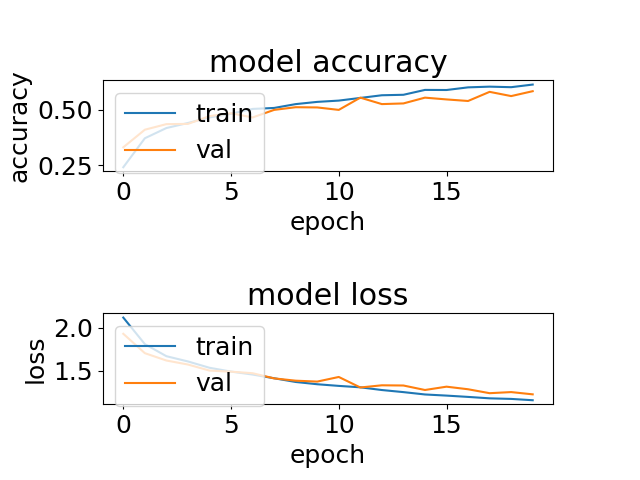
\includegraphics[width=8cm]{5k.png}}}
\qquad
\subfloat[10k Dataset]{{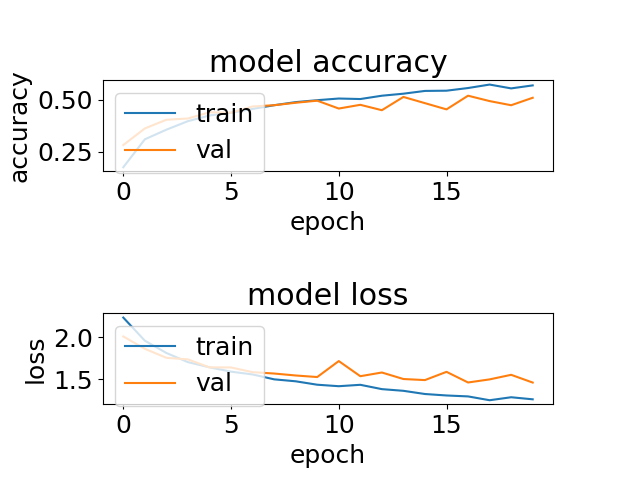
\includegraphics[width=8cm]{10k.png}}}
\qquad
\subfloat[20k Dataset]{{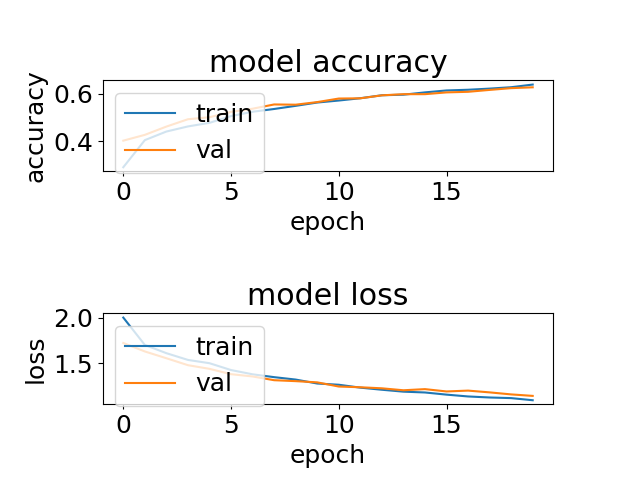
\includegraphics[width=8cm]{20k.png}}}
\qquad
\subfloat[40k Dataset]{{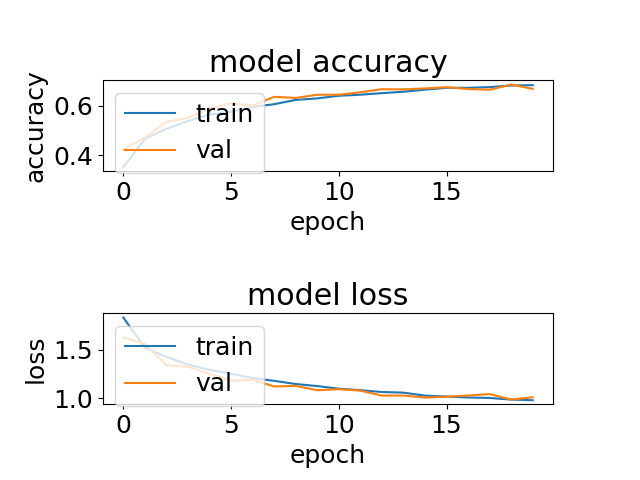
\includegraphics[width=8cm]{40k.png}}}
\qquad
\end{figure}
\subsubsection{iv}
As we vary the L1 penalty,  the accuracy fluctuates quite a bit.  With 0, our accuracy actually increases in terms of the training and test data but as we increase the penalty,  the accuracy become worse and worse.  Using a large L1 value such as 10, out accuracy is terrible got both our training and test datasets. This could be due to the fact that by increasing th L1 penalty, the CNN attempts to prevent overfitting more and more and hence begins underfitting the data with larger values of L1 since the weights are so high.
\begin{figure}[h]
\centering
\subfloat[L1 = 0]{{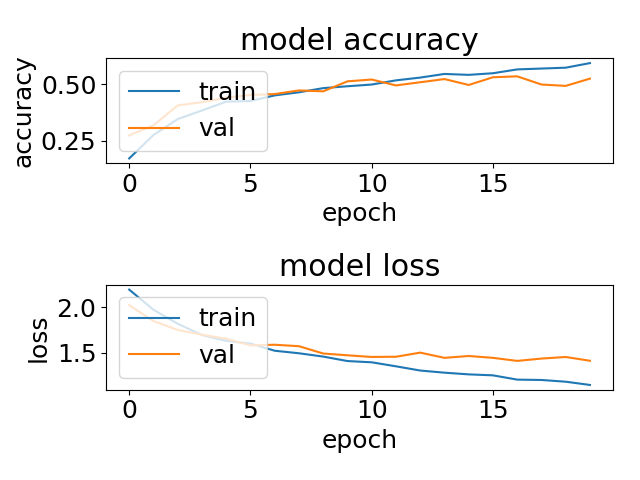
\includegraphics[width=8cm]{L0.png}}}
\qquad
\subfloat[L1 = 0.0001]{{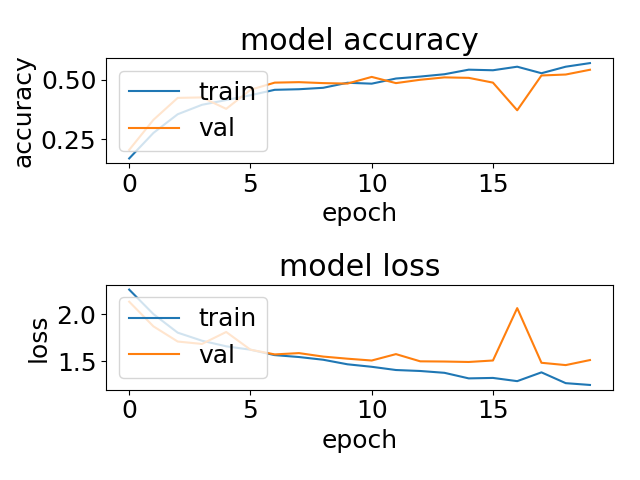
\includegraphics[width=8cm]{L1.png}}}
\qquad 
\subfloat[L1 = 0.001]{{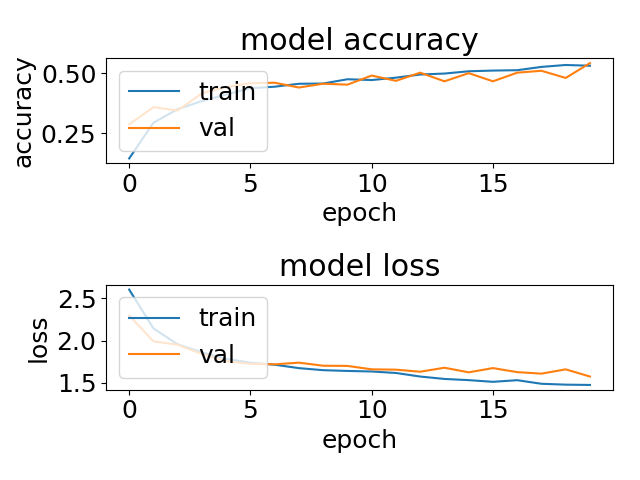
\includegraphics[width=8cm]{L2.png}}}
\qquad
\subfloat[L1= 0.01]{{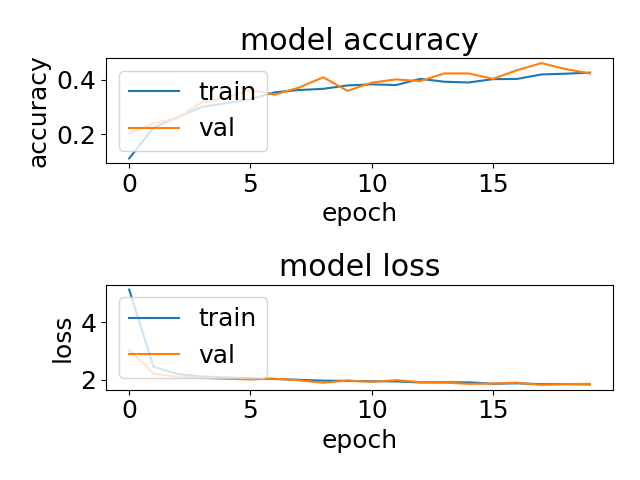
\includegraphics[width=8cm]{L3.png}}}
\qquad
\subfloat[L1 = 0.1]{{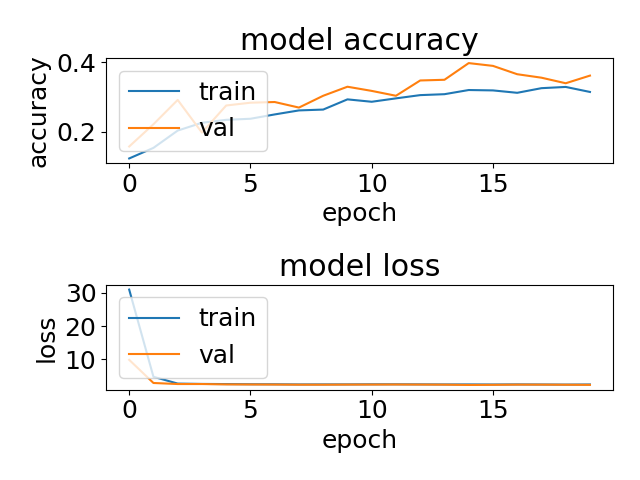
\includegraphics[width=8cm]{L4.png}}}
\qquad
\subfloat[L1 = 1]{{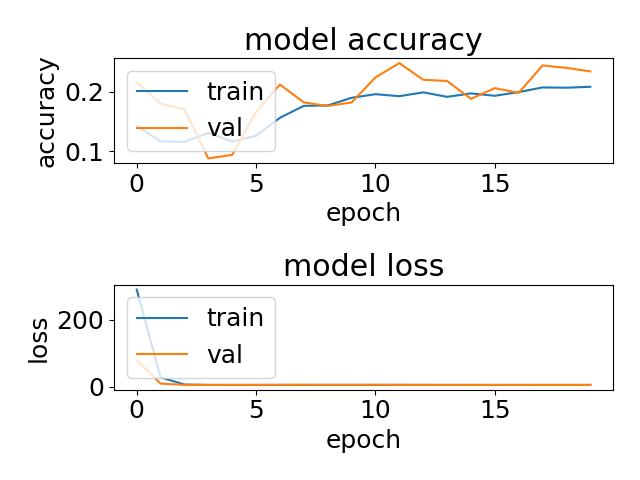
\includegraphics[width=8cm]{L5.png}}}
\qquad
\subfloat[L1 = 10]{{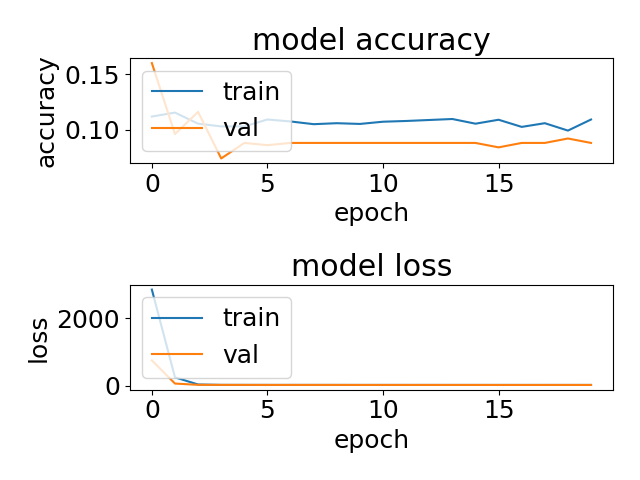
\includegraphics[width=8cm]{L6.png}}}
\end{figure}
\clearpage
\subsection{C}
\subsubsection{i}
In the code below, I commented out the layers that perform striding and instead added in max-pooling layers instead.
\begin{verbatim}
model = keras.Sequential()
        model.add(Conv2D(16, (3, 3), padding='same', input_shape=x_train.shape[1:], activation='relu'))
        # model.add(Conv2D(16, (3, 3), strides=(2, 2), padding='same', activation='relu'))
        model.add(MaxPooling2D((2,2), padding='same'))
        model.add(Conv2D(32, (3, 3), padding='same', activation='relu'))
        model.add(MaxPooling2D((2,2), padding='same'))
        # model.add(Conv2D(32, (3, 3), strides=(2, 2), padding='same', activation='relu'))
        model.add(Dropout(0.5))
        model.add(Flatten())
        model.add(Dense(num_classes, activation='softmax', kernel_regularizer=regularizers.l1(i)))
        model.compile(loss="categorical_crossentropy", optimizer='adam', metrics=["accuracy"])
        model.summary()
\end{verbatim}

\subsubsection{ii}
When using max-pooling, the total number of parameters reported by keras is 25,578, with 20,490 of these parameters coming from our dense layer.  The time per step for this network is 5ms/step which is lower than the 7ms/step of the original network. This speedup does come at a cost though, the accuracy of our models is affected, with the accuracy of our network on the training data dropping to .55 from .60 but it doesn't seem to affect the test data, with the test data having a score of .49 using max-pooling while the original reported the exact same score.  The reason the training time has changed is due to reducing the computational load. Max pooling essentially reduces the size of the output of the convolutional layers which in turn reduces the number of parameters in the network hence reducing the load. This is why we've less parameters in our model in comparison to our original model.
\subsection{D}
To achieve over 70\% accuracy using the given architecture for the Convolutional network, I had to increase the number of epochs by a factor of 3, essentially tripling the time required to train it.  Adding more layers affects the network in difference ways. \\\\In regards to  prediction performance,  adding more layers doesn't necessarily mean better performance.  If the individual layers are thinner,  we don't get a performance uplift because overall we've less parameters to train on so our performance is also limited.  In this network we've got a total of 23,314 parameters as compared to the over 30,000 parameters in our original network.
\\\\In terms of over/under fitting,  adding more layers can lead to over-fitting as we're extracting too many features from the dataset, which can lead to false positives.  \\\\ In terms of the amount of training data and time taken to trade,  I had to use the 40K dataset and even then it took 3x as long to train the data to get over 70\% accuracy.  Adding more layers again doesn't guarantee we can use less data and train for less time overall.  It depends on how well the layers can extract data from the dataset so that we can train for less time overall and need less data. 
\end{document}
